%\documentclass[journal]{vgtc}                % final (journal style)
\documentclass[review,journal]{vgtc}         % review (journal style)
%\documentclass[widereview]{vgtc}             % wide-spaced review
%\documentclass[preprint,journal]{vgtc}       % preprint (journal style)

%% Uncomment one of the lines above depending on where your paper is
%% in the conference process. ``review'' and ``widereview'' are for review
%% submission, ``preprint'' is for pre-publication, and the final version
%% doesn't use a specific qualifier.

%% Please use one of the ``review'' options in combination with the
%% assigned online id (see below) ONLY if your paper uses a double blind
%% review process. Some conferences, like IEEE Vis and InfoVis, have NOT
%% in the past.

%% Please note that the use of figures other than the optional teaser is not permitted on the first page
%% of the journal version.  Figures should begin on the second page and be
%% in CMYK or Grey scale format, otherwise, colour shifting may occur
%% during the printing process.  Papers submitted with figures other than the optional teaser on the
%% first page will be refused. Also, the teaser figure should only have the
%% width of the abstract as the template enforces it.

%% These few lines make a distinction between latex and pdflatex calls and they
%% bring in essential packages for graphics and font handling.
%% Note that due to the \DeclareGraphicsExtensions{} call it is no longer necessary
%% to provide the the path and extension of a graphics file:
%% 
\includegraphics{diamondrule} is completely sufficient.
%%
\ifpdf%                                % if we use pdflatex
  \pdfoutput=1\relax                   % create PDFs from pdfLaTeX
  \pdfcompresslevel=9                  % PDF Compression
  \pdfoptionpdfminorversion=7          % create PDF 1.7
  \ExecuteOptions{pdftex}
  \usepackage{graphicx}                % allow us to embed graphics files
  \DeclareGraphicsExtensions{.pdf,.png,.jpg,.jpeg} % for pdflatex we expect .pdf, .png, or .jpg files
\else%                                 % else we use pure latex
  \ExecuteOptions{dvips}
  \usepackage{graphicx}  % allow us to embed graphics files
  \DeclareGraphicsExtensions{.eps}     % for pure latex we expect eps files
\fi%

%% it is recomended to use ``\autoref{sec:bla}'' instead of ``Fig.~\ref{sec:bla}''
\graphicspath{{figures/}{pictures/}{images/}{./}} % where to search for the images

\usepackage{microtype}                 % use micro-typography (slightly more compact, better to read)
\PassOptionsToPackage{warn}{textcomp}  % to address font issues with \textrightarrow
\usepackage{textcomp}                  % use better special symbols
\usepackage{mathptmx}                  % use matching math font
\usepackage{colortbl}
\usepackage{times}                     % we use Times as the main font
\renewcommand*\ttdefault{txtt}         % a nicer typewriter font
\usepackage{cite}                      % needed to automatically sort the references
\usepackage{tabu}                      % only used for the table example
\usepackage{booktabs}                  % only used for the table example

\newcommand{\wrong}[1]{\textcolor{red}{#1}}
\newcommand{\lang}[1]{\textcolor{orange}{#1}}


\newcommand\Tstrut{\rule{0pt}{2.6ex}}         % = `top' strut
\newcommand\Bstrut{\rule[-0.9ex]{0pt}{0pt}}   % = `bottom' strut

%% We encourage the use of mathptmx for consistent usage of times font
%% throughout the proceedings. However, if you encounter conflicts
%% with other math-related packages, you may want to disable it.

%% In preprint mode you may define your own headline.
%\preprinttext{To appear in IEEE Transactions on Visualization and Computer Graphics.}

%% If you are submitting a paper to a conference for review with a double
%% blind reviewing process, please replace the value ``0'' below with your
%% OnlineID. Otherwise, you may safely leave it at ``0''.
\onlineid{0}

%% declare the category of your paper, only shown in review mode
\vgtccategory{Research}
%% please declare the paper type of your paper to help reviewers, only shown in review mode
%% choices:
%% * algorithm/technique
%% * application/design study
%% * evaluation
%% * system
%% * theory/model
\vgtcpapertype{please specify}

%% Paper title.
\title{Narvis: How to Explain An Advanced Visualization Design}

%% This is how authors are specified in the journal style

%% indicate IEEE Member or Student Member in form indicated below
\author{Roy G. Biv, Ed Grimley, \textit{Member, IEEE}, and Martha Stewart}
\authorfooter{
%% insert punctuation at end of each item
\item
 Roy G. Biv is with Starbucks Research. E-mail: roy.g.biv@aol.com.
\item
 Ed Grimley is with Grimley Widgets, Inc.. E-mail: ed.grimley@aol.com.
\item
 Martha Stewart is with Martha Stewart Enterprises at Microsoft
 Research. E-mail: martha.stewart@marthastewart.com.
}

%other entries to be set up for journal
\shortauthortitle{Biv \MakeLowercase{\textit{et al.}}: Global Illumination for Fun and Profit}
%\shortauthortitle{Firstauthor \MakeLowercase{\textit{et al.}}: Paper Title}

%% Abstract section.
\abstract{nothing here%
} % end of abstract

%% Keywords that describe your work. Will show as 'Index Terms' in journal
%% please capitalize first letter and insert punctuation after last keyword
\keywords{Narrative visualization, visual encoding explanation, }

%% ACM Computing Classification System (CCS). 
%% See <http://www.acm.org/class/1998/> for details.
%% The ``\CCScat'' command takes four arguments.

\CCScatlist{ % not used in journal version
 \CCScat{K.6.1}{Management of Computing and Information Systems}%
{Project and People Management}{Life Cycle};
 \CCScat{K.7.m}{The Computing Profession}{Miscellaneous}{Ethics}
}

%% Uncomment below to include a teaser figure.
\teaser{
  \centering
  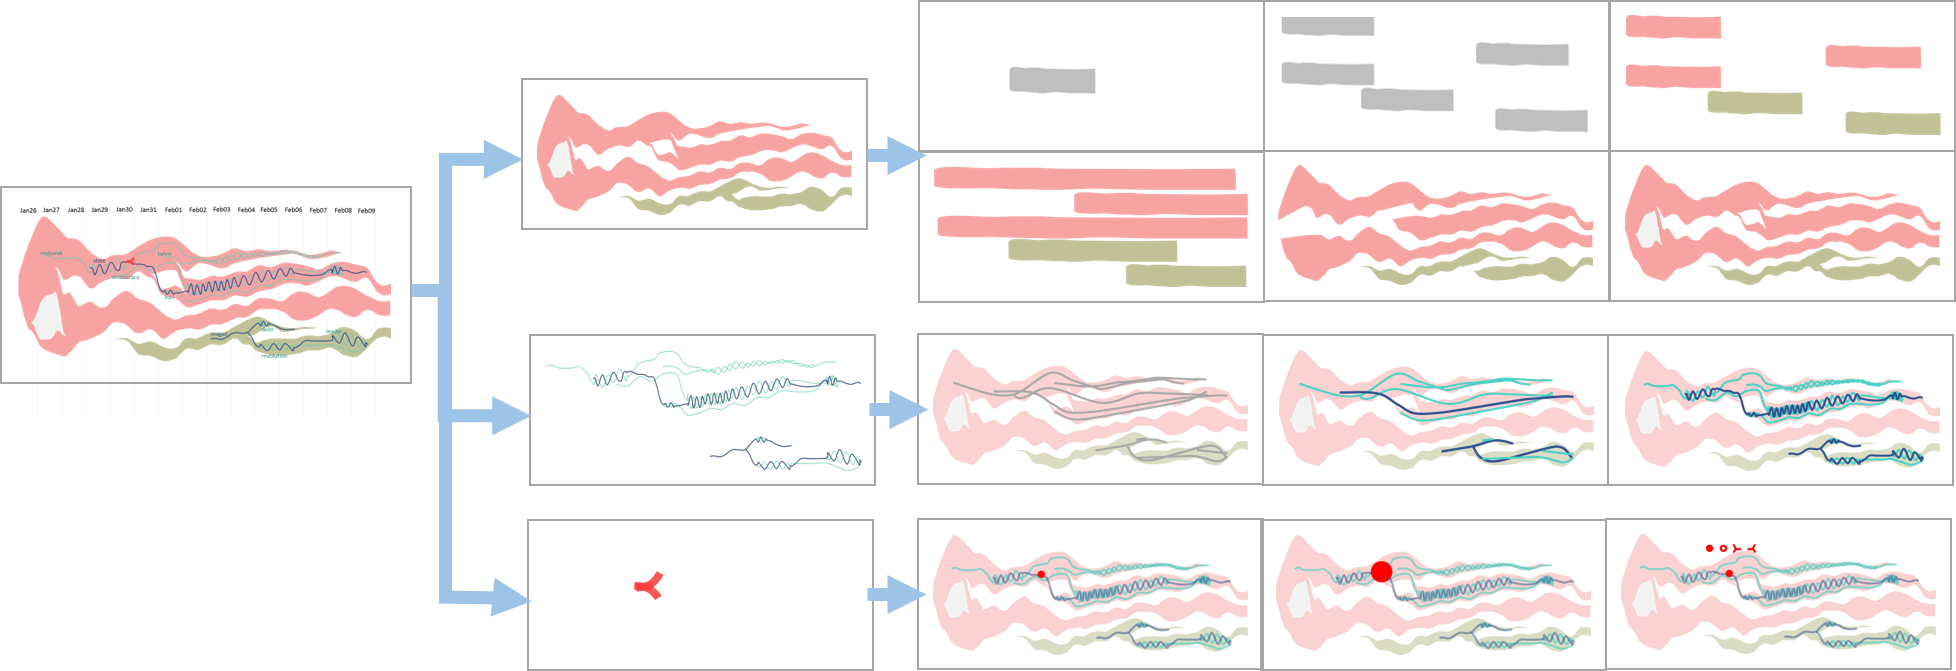
\includegraphics[width=\linewidth]{Picture1}
  \caption{we don't have the system , we have nothing to add here at this time point}
	\label{fig:teaser}
}

%% Uncomment below to disable the manuscript note
%\renewcommand{\manuscriptnotetxt}{}

%% Copyright space is enabled by default as required by guidelines.
%% It is disabled by the 'review' option or via the following command:
% \nocopyrightspace

\vgtcinsertpkg

%%%%%%%%%%%%%%%%%%%%%%%%%%%%%%%%%%%%%%%%%%%%%%%%%%%%%%%%%%%%%%%%
%%%%%%%%%%%%%%%%%%%%%% START OF THE PAPER %%%%%%%%%%%%%%%%%%%%%%
%%%%%%%%%%%%%%%%%%%%%%%%%%%%%%%%%%%%%%%%%%%%%%%%%%%%%%%%%%%%%%%%%

\begin{document} 

%% The ``\maketitle'' command must be the first command after the
%% ``\begin{document}'' command. It prepares and prints the title block.

%% the only exception to this rule is the \firstsection command
\maketitle
 
\section{Introduction} %for journal use above \firstsection{..} instead
For data with complicated structure, naive data visualization like bar chart and pie chart maybe unsatisfying for a comprehensive display. By introducing metaphors borrowed from nature \cite{cao_whisper:_2012,huron_visual_2013}, applying carefully designed layout algorithms\cite{wu_opinionflow:_2014,chi_morphable_2015}, and sophisticatedly combining existing visualizations\cite{zhao_x0023;fluxflow:_2014}, novel visual presentations help people identify patterns, trends and correlations hidden in data. However, these advanced visualizations are usually not intuitively recognizable. Users need to go through some training, for example, reading a long and boring literal description, before they grasp the knowledge required to understand and freely explore a visualization.\par
What is more, even designers of these advanced visualizations suffer when they are required to introduce their design, especially when the visual encoding has complicated logic dependency, or when their audience have little prior knowledge about visualization techniques.\par
As a result, these advanced visualization technologies, in spite of
the fact that their utility has been verified by domain experts from various fields, gain little exposure outside the visual community. Main stream media is still dominated by naive visualizations, such as bar charts, pie charts and so on.

For a visualization, its core design space can be described as the orthogonal combination of two aspects: graphical elements called marks and visual channels to control their appearance\cite{munzner_visualization_2014}. But why the explanation of these two things is so complicated? 

This problem mainly arises from the fact that advanced visualization designs usually attempt to delivery a great amount of information. First, it would overload an audience if we inundated them with all the information at one time. Second, even if we tried to explain it sequentially, considering the logic dependency existing among visual elements, an improper explanation could totally confuse the audience. For example, in a node link diagram, a node should be introduced before the links connecting it. In an advanced visualization design, which has more components than just nodes and links, it is challenging to identify a proper explaning oder. Third, when digesting such a considerable amount of information, audiences can easily get distracted or forget previous information.   

Thus, to better introduce an advanced visualization, we should convey its information sequentically and in a specific order. Attention guidance and reminders are also needed to make sure that audiences are following this order, not getting distracted or forgetting previous information.

Narrative, which means “connected events presented in a sequence”, has long been used to share complex information. \cite{schmidt_living_2017}As the data visualization field is maturing, many researchers have moved their focus from analysis to presentation, making narrative data visualization an emerging topic\cite{kosara_storytelling:_2013}. Many efforts have been
made to define, classify, and provide design suggestions for narrative data visualization\cite{segel_narrative_2010,hullman_deeper_2013,gershon_what_2001}. Some visualization systems have already incorporated narrative modules into their design\cite{eccles_stories_2007,bryan_temporal_2016}. However, current work is mainly focused on communicating the conclusion of analyses, rather than guiding the audience how to read a visualization. 

Here, we present a prototype to adopt narrative techniques to create a visual encoding explanation. We
ground our work on text visualization designs, but we believe our findings and our system generalize to other types of visualization. Based on our analysis of the structure, logic dependency, and visual distraction existing in a visualization design, we develop an authoring tool to decompose a visualization, reorganize extracted visual elements, and explain their visual encodings one by one through animated transition in the form of slideshow. Through incorporating a narrative sequence, appropriate chunks of information, rather than all the information, is delivered to the audience at one time, effectively avoiding information overload. Reminders, such as questions, summarizations and repetitions are woven into the narrative sequence to enhance the audience’s memory while visual attention guidance, such as flickering, highlighting, and morphing are used to lead their attention to newly added information. (字数超了就删掉)

To the best of our knowledge, this is the first attempt to explain visual encoding with narrative. Our contributions are as below: 1). A paradigm for decomposing visualizations. It analyzes the hierarchical structure of its components, the relationships between components, and visual distraction existing. 2) A framework for explaining visualization design, which is the result of consulting theory from graphical perception process, techniques in narrative visualization, various attention cues in animation, and empirical observations of numerous visualization designs. 3) An authoring tool to generate and edit the narrative visual encoding explanation
 We conjecture our work can motivate and enable people to use more advanced visualization designs, supporting the democratization of data visualization.
 

\section {Related work}
In this section, we provide an overview of prior research around the analysis of narrative structure in data visualization, animation in data visualization, and existing authoring tools for narrative visualizations.\par
\subsection{Structure of Narrative Data Visualization}
Narrative is as old as human history. [cite something] People in the fields of literature, comics \cite{cohn_visual_2013} and cinema \cite{schmidt_living_2017} have gone to great lengths to analyse the sequencing and forms of grouping used in a narrative, as well as how they affect the meaning a narrative tries to deliver. \par
Some people believe that work from other fields can inspire researchers in the visual data community. Amini et al\cite{amini_understanding_2015} borrow concepts from comics \cite{cohn_visual_2013} to classify and analyse the structure of data videos. Wang et al \cite{wang_animated_2016} adopt two representative tactics, time-remapping and foreshadowing, from cinematographers to organize a narrative sequence for visualizing temporal data. \par
Other researchers, on the other side, focus on the narrative structures exclusively for data visualization. \par
Satyanarayan and Heer, through interviews with professional journalists\cite{satyanarayan_authoring_2014}, define the core abstractions of narrative data visualization as state-based scenes, visualization parameters, dynamic graphical and textual annotations, and interaction triggers. Hullman et al\cite{hullman_deeper_2013}, by identifying the change in data attributes, propose a graph-driven approach to automatically identify effective narrative sequences for linearly presenting a set of visualizations. \par
These works, however, rarely discuss the narrative structures used for visual encoding scheme, which is fundamental to a visualization. We hope our work can fill this gap.\par
\subsection{Animation for data visualization}
There is a wide discussion about the effects of animation when used in a data visualization environment.\par 
Animation can facilitate the cognitive process. Heer and Robertson \cite{heer_animated_2007-1} confirm the effectiveness of animation when relating data visualizations backed by a shared dataset. Ruchikachorn et al\cite{ruchikachorn_learning_2015}, going a step further, design morphing animations which bridge the gap between a familiar visualization and an unfamiliar one, thus introducing a new visualization design through animation. Graphdiaries \cite{bach_graphdiaries:_2014} uses animation to help audiences track and understand changes in a dynamic visualization. \par
On the other hand, animation can be an effective tool to attract and guide visual attention. Huber et al \cite{huber_visualizing_2005} study the perceptual properties of different kinds of animation, as well as their effects on human attention. Waldner et al \cite{waldner_attractive_2014} focus on a specific animation: flicker. By dividing the animation into an “orientation stage” and an “engagement stage”, they strike a good balance between the attraction effectiveness and annoyance caused by flickering. \par
It is, however, noteworthy that animation, in spite of all the advantages mentioned above, can bring about negative effects when used improperly\cite{robertson_effectiveness_2008}. Our work is based on the results of these researches, which provide a guideline on how to implement animations in our system.\par
\subsection{Authoring tools for narrative visualization}
The extensive needs of data communication exist not only in the data visualization field but also in journalism, media, and so on. This has motivated researchers to investigate ways for authoring narrative visualization. \par
User experience is of great concern when utilizing an authoring tool. Sketch story \cite{lee_sketchstory:_2013}, with its freeform sketch interaction, provides a more engaging way to create and present narrative visualization. Dataclips \cite{amini_authoring_2017}lowers the barrier of crafting narrative visualization by providing a library of data clips, allowing non-experts to be involved in the production of narrative visualization. \par
However, it is information delivery that is the core consideration of an authoring tool. Existing authoring tools usually choose a specific type of narrative visualization based on the information type. \cite{amini_authoring_2017}Meanwhile, integrating an authoring tool for narrative visualization with a  data analysis tool has become a trend since it effectively bridges the gap between data analysis and data communication. \cite{eccles_stories_2007,bryan_temporal_2016,lee_more_2015}\par 
These tools offer inspiring user interaction design as well as good examples to implement narrative visualization. However, they treat visual encodings as cognitively obvious attributes that can be universally recognized without a formal introduction, making them inapplicable in our case. \par
\subsection{Decompose a data visualization}
Clarifying the design space of a data visualization can help people get a better understanding of how it is constructed. Tamara \cite{munzner_visualization_2014} proposes that it "can be described as an orthogonal combination of two aspects: graphical elements called marks and visual channels to control their appearance". Borrowing the concept of physical building blocks such as Lego, Huron et al \cite{huron_constructive_2014} extends the design space of a data visualization, defining the components of a data visualization as a token, token grammar, environment and assembly model.\par 
Such theoretical work, although varying from one to another, motivate the designers of visualization tools to contribute efficient high-level visualization systems rather than low-level graphical systems.\cite{bostock_protovis:_2009,mendez_ivolver:_2016} \par 
On the other hand, theoretically identifying the basic components of a data visualization enables people to physically extract them, and remap them to an alternative design without involving any programming work. Harper and Agrawala \cite{harper_deconstructing_2014} contribute a tool that extracts visual variables from existing D3 visualization designs to generate a new design.Huang et al\cite{Huang:2007:SUI:1284420.1284427} propose a system that recognizes and interprets imaged
infographics from a scanned document. Revision\cite{savva_revision:_2011} applies computer vision method to recognize the types, marks, encodings of a data visualization, and allows the users to create a new design based on these data. \par 
However, these decomposing methods exclusively focus on simple visualization designs, such as bar chart, line chart, dot chart, and are not applicable for advanced visualization designs, which assemble miscellaneous visualization approaches to realize a novel presentation. Moreover, these methods are put forward for the purpose of constructing a visualization, instead of explaining an already existing one, thus giving no consideration for graphical perception process and visual attention shift.\par 

\begin{table}[tb]
  \caption{A survey of visualization designs published on TVCG: 2007-2017}
  \label{tab:vis_papers}
  \scriptsize%
	\centering%
  \begin{tabu}{%
	r|
	*{11}{c|}%
	*{1}{r}%
	}
  \toprule
\textbf{sum} & \textbf{ } & \textbf{ } & \textbf{ } & \textbf{ } & \textbf{ } & \textbf{ } & \textbf{ } & \textbf{ } & \textbf{ } & \textbf{ } & \textbf{ } \\
  \bottomrule
\end{tabu}%     
\end{table}

\section{Analysis of a visualization} 
To better inform the crafting of a narrative explanation, we survey more than 60 papers about data visualization design that published in journals with high impact and have high citations. Based on our survey, we propose a model that try to decompose the structure of an advanced visualization, as well as to identify correlations and visual distractions existing between different compositions. At the same time, borrowing heavily from the existing perceptual and cognitive theory, we put forward some suggestions for the design of narrative visualization explanation. 
\par
\begin{figure}
 \centering % avoid the use of \begin{center}...\end{center} and use \centering instead (more compact)
 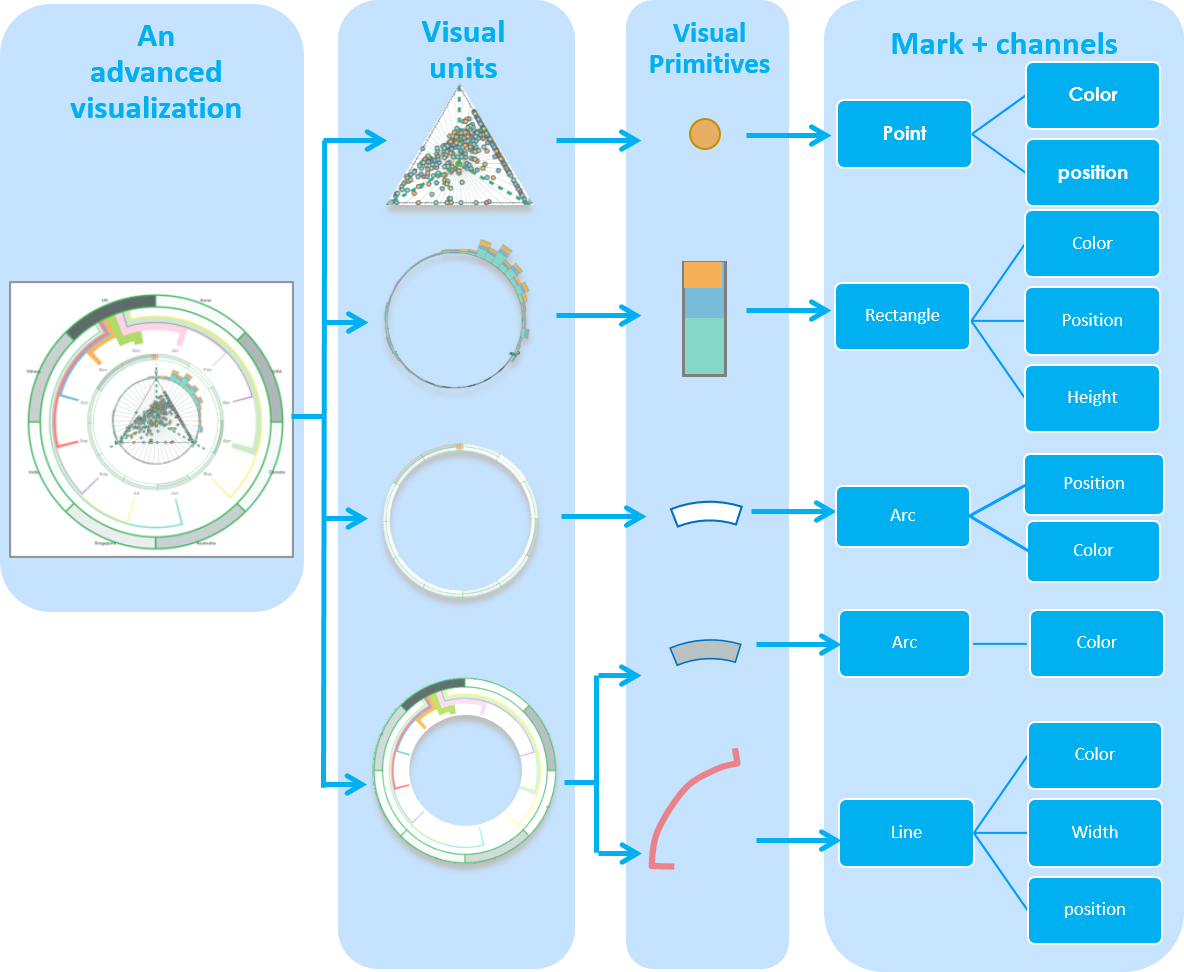
\includegraphics[width=\columnwidth]{Picture2}
 \caption{An example of the hierarchical structure of a visualization, Opinion Seer\cite{wu_opinionseer:_2010}}
 \label{fig:sample}
\end{figure}
\subsection{Compositions of a visualization}
Previous works have proven that learning by constructin is effective for grasping new knowledge.\cite{huron_constructive_2014, chapman_constructive_1988}  We incorporate the lessons from previous work\cite{munzner_visualization_2014, huron_constructive_2014, chi_taxonomy_2000}  with our observation, define the compositions of a visualization. 
\wrong{maybe define what is an advanced visualization design????}
\subsubsection{Hierarchical structure}
We propose a model that decomposes a visualization into three levels of structure: visual primitives, visual units, and then an advanced visualization design. A visual primitive is one graphic element, also called as mark\cite{munzner_visualization_2014} or token\cite{huron_constructive_2014}, with all the visual channels controlling its appearance. For instance, a point whose position and color are encoded is a visual primitive. It is the combination of one mark, point, with two visual channels, color and position. A visual unit is the combination of visual primitives. It is also the smallest functional unit of a visualization. A scatter plot, which groups the points mentioned above, is a visual unit. A node-link diagram, which is also a visual unit, is consist of two visual primitives, points mentioned above and lines whose position and color are encoded.  An advanced visualization can be treated as the combination of visual units. 

\par
\begin{figure}[tb]
 \centering % avoid the use of \begin{center}...\end{center} and use \centering instead (more compact)
 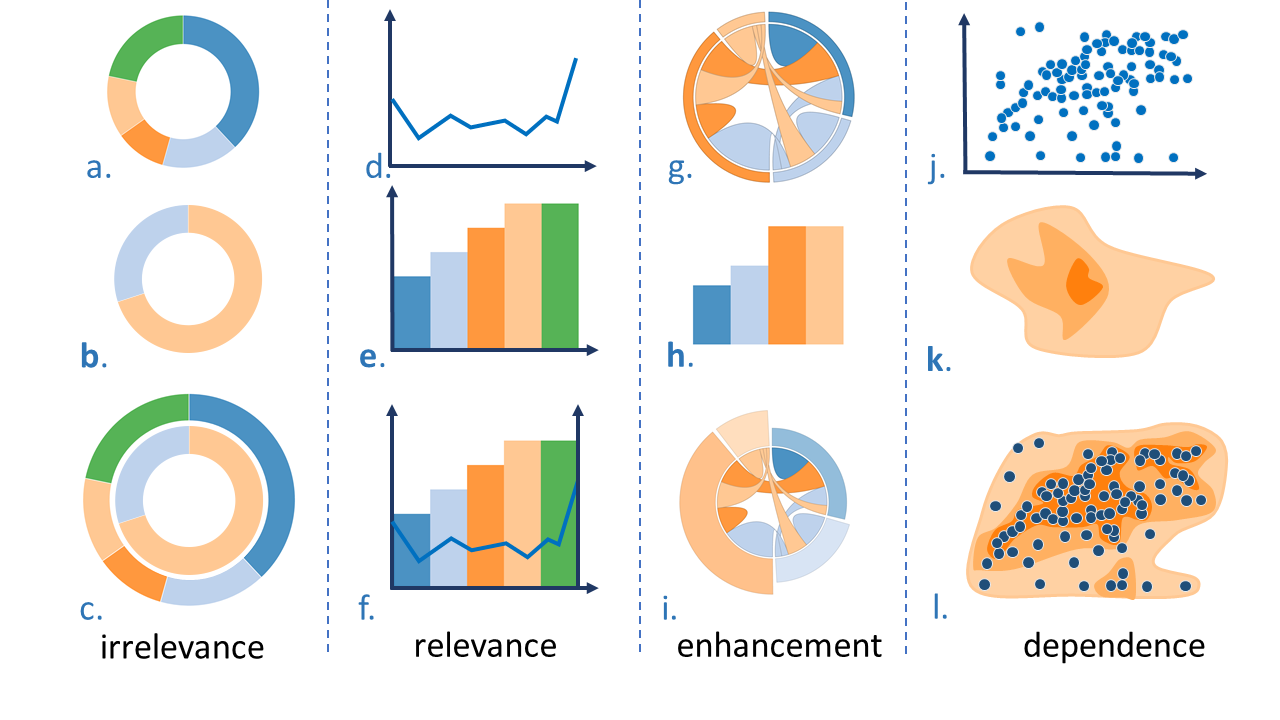
\includegraphics[width=\columnwidth]{unit_relationship}
 \caption{Illustration of the 4 types of relationship between visual units}
 \label{fig:sample}
\end{figure}




\begin{table}[tb]
  \small
  \centering
  \begin{tabular}{p{0.8cm}|p{2.1cm}|p{2.1cm}|p{2.1cm}}
  \toprule
  &\textbf{Radial} & \textbf{Linear / Parallel} & \textbf{Metric-dependent} \Tstrut\Bstrut  \\ 
  \midrule
  \textbf{Line} & & Line Chart & \\ 
  \midrule
  \textbf{Area} & &Area Graph  & Treemap \\ 
  \midrule
  \textbf{Bar} &Radial Bar Chart & Bar Chart & \\
  \midrule
  \textbf{Dot} & &Scatter Plot &Bubble Map \\
  \midrule
  \textbf{Wedge} & Pie Chart &Arc Diagram & \\
  \midrule
  \textbf{Link} &Chord Diagram &Parallel Coordinates &Node-link Diagram \\
  \midrule
  \textbf{Text} & &Parallel Tag Cloud [] &Word Cloud \\
  \midrule
  \textbf{Image} & &Heatmap Matrix &Heatmap \\

  \bottomrule

  \end{tabular}
  \vspace{1mm}
  \caption{A summary of visual units.}
  \label{tab:unit}
\end{table}


\subsubsection{Relationships between visual units}
An advanced visualization is often the combination of several visual units. Through observing the approaches people apply to design new visualizations, \wrong{we define four types of relationship between visual units in our model, \textbf{need a table for it}}: irrelevance, relevance, enhancement, and dependency. \par
\textbf{Irrelevance} refers to that two visual units have no correlations in their visual encodings. It is a bi-directional relation. As in \textbf{figure1a}, 2 donut charts are applied to illustrate the distribution of age and gender groups respectively in a population. They are put together just for space-efficiency and there is no correlation between these two charts. \par
\textbf{Relevance} refers to that two visual units share some encoding scheme, and it is a bi-directional relation. For example, in \textbf{figure 1b}, bar chart and line chart show the same encoding of horizontal position. According to our survey, color and position are the most commonly shared visual encodings, which might be the result that color and position usually encoded with simple while crucial information. \par
\textbf{Enhancement} is an one-way relationship. If one visual unit A is the enhancement of another visual unit B, it means that A is imported to B, replaces some graphic elements of B and thus enables the representation of some data attributes that B alone fails to convey. Suppose there are 5 types of area in a park. A bar chart illustrates their average price per unit area, a chord diagram illustrates how passengers travel through each area. Then, as in \textbf{figure 1c}, the bar chart take the place of node segments in chord diagram, resulting in a novel and informative visualization. Some actual examples are the heat map mapped upon the steams in a theme river\cite{wu_opinionseer:_2010}  and usage of glyphs to enhance the meaning of nodes in a multidimensional scaling plot.\cite{chen_peakvizor:_2016}\par
\textbf{Dependence} is an one-way relationship. If one visual unit A is dependent on B, it means that A is added to B to reveal some information that results from the visualization B adopts to a dataset. The biggest difference between "\textbf{enhancement}" and "\textbf{dependence}" is that \textbf{enhancement} illustrate the data attributes in the data set, while \textbf{dependency} reveals the new knowledge we obtain from adopting a visualization a dataset. For example, in \textbf{figure xxx}, a multiple dimensional scaling (MSD) map shows the similarity between each restaurants in a city. A heat map is then added to the MSD map to show the most common type of restaurants, which information can hardly be obtained from the dataset but quite evident from the previous visualization. 
\subsubsection{Correlations between visual primitives}
The inner relationship between visual primitives is relatively simple.
A visual unit, which is the smallest function unit in a visualization, rarely have more than 2 visual primitives. And the relationship between the 2 visual primitives, if there are two, are quite obvious. The encoding of one primitive always has a high dependency on the encoding of another primitive. For example, in a chord diagram, the encoding of the arcs should be explained before the line connecting them. 

\subsubsection{Correlations between visual channels}
The relationship between channels might be the most complicated relationship in our model. Since different channels are encoded with different information, they are usually separated and have no logic dependency upon others. However, an arbitrary explaining order of visual channels may lead to an unefficient information delivery, especially when a mark has multiple channels, which is common in an advanced visualization. 

Therefore, we define two metrics to order the explaining of visual channels: \textbf{the complexity of their encoded information} and \textbf{saliency of their visual appearance}.

First, a proper explanation should follow the order of decreasing visual saliency.\cite{cleveland_graphical_1984} Even though different channels have intrinsically different perceptual salience and channel with high salience will suppress the expression of other, such salience strength can be influenced in a task-dependent manner. \cite{nothdurft_salience_2000} By introducing the channel with high saliency first, we remove it from the task list in our mind, decrease its saliency and give other channels more chance to attract limited human attention. (maybe introduce some concepts such as salience map, pre-attentive stage, and focused attention stage) \par
 Second, we should follow the order of increasing complexity. “Easy to difficult” practice has been long used and confirmed to be effective for learning new tasks\cite{bliss_effects_1992}.\par
 Based on our survey, there are five common visual channels: color hue, size, position, shape, color saturation. Sorted in the increasing complexity order, it is color hue-color saturation-position-size-shape, while sorted in the decreasing visual saliency order, it is position-color hue-size-shape-color saturation \cite{munzner_visualization_2014,cleveland_graphical_1984}.  \par
In our system, we choose position-color hue-color saturation-size-shape as a trade-off between these two metrics. But we do allow and recommend the users to define their preferable sequence based on their situation. \par
\subsection{Analysis of existing visual distraction}
\textbf{add a fig}
From our observation, we identify two kinds of visual distractions: visual distraction from context and visual distraction from sibling channels (sibling channels refer to the channels belonging to the same mark). \par
\textbf{Visual distraction from the context}: This kind of distraction has been widely discussed in the field of object detection and human visual attention. \cite{nothdurft_salience_2000, standage_modelling_2005}Its intensity is mainly  determined by spatial distance and appearance similarity. \cite{wolfe_guided_1994}For example, when we try to focus on a green rectangel, a red triangel near by it can lead to visual distraction. And the intensity of such distraction is determined by the distance and the appearance similarity between the two graphics. Focus + Context, which might be the most popular techniques for this problem, make uneven use of graphic resources to discriminate focus from their context. At the same time, adding dynamic changes to focus elements has also been demonstrated as effective under various conditions\cite{waldner_attractive_2014}. 

\textbf{Visual distraction from sibling channels}: A visual primitive usually has more than one visual channels. Thus, when recognizing one primitive, the channels with high visual saliency can significantly influence the expression of other channels. For example, color can be a strong noise when focus is supposed to be the shape.

\subsection{Design considerations of narrative sequence}
\textbf{Channels}: As discussed in section 3.1.4, when explaining channels, we should take information complexity as well as visual saliency into account. 

As for one channel, the narrative explanation depends on the type of the channel. As defined previous work, therer namely, whether it is a magnitude channel, which expresses ordered data attributes, or an identity channel, which expresses category data attributes. For a magnitude channel, two extreme examples will be enough for explaining, while for an ordered channel, introducing each category one by one might be a better option.\par
\textbf{Units}: As discussed in section 3.1.2, there are four types of relationships between visual units, and they will influence the order of a narrative explanation. Thus, we display the correlations between units in a tree diagram where a child node is the enhancement/dependence of its parent node and sibling nodes have logic dependences. When explaining these visual units, we can simply obey a deep first search (DFS) order to visit all the visual units.\par
\textbf{Non-linear sequence}: so far, all the narrative explanation we discussed is linear. We move from one channel to another channel, then from one primitive to another primitive, then from one unit to another unit. However, the fact is that no one likes to read a lengthy, extremely detailed instruction. A good narrative explanation should include non-linear design, allowing users to skip uninterested, go back to previous information and freely switch between different parts. Also, users should be allowed the flexibility to choose explanations at different levels of details, more specifically, a detailed mode, a normal mode, an abstract mode. \par
\section{Narvis: Authoring Narrative Explanation for Data Visualization}
\subsection{An overview}
Narvis is aimed to offer an efficient, expressive and friendly authoring tool for the experts in data visualization, help them create a slide show for the purpose of introducing an advanced visualization design to general audience.  \par
Narvis is consist of three phase: Automatic Analysis Phase, Human Editing Phase, Reviewing Phase.\par
In Automatic Analysis Phase, the system will automatically extract the graphical elements in the input visualization with an algorithm based on edge detection. These graphic elements will be classified based on their visual appearance, such as the area, color, the number of corners. Input text description will also be classified based on the keywords we pre-defined in our system. \par 
In Human Editing Phase, users will modify the output from the Automatic Analysis Phase, call the templates we offer, and craft a slide show to introduce an advanced visualization. \par 
In Reviewing Phase, reviews can assess the slide show generated in Human Editing Phase. Their feedback, more specifically, their click activity and comments, will be recorded and send to the Human Editing Phase, helping improve the quality of the slide show. 
\subsection{Design consideration}
Hence, we settle on six design considerations(DCs) for this authoring tool. Our premise is that the user is familiar with the visual encodings of a visualization design but unclear how to educate his audiences in an efficient way. \par
\textbf{DC1. Clear structure and organized narrative sequence.}\par
The complicated relationship, spatial and logical alike,  between different graphic elements is one of the biggest barriers that impedes a smooth communication of visual encoding scheme. By encouraging users to refine the clusters of graphic elements, to figure out relationship between visual units by editing a unit tree, and to modify the narrative templates we offered, we aim at motivating users to sort out the structure of a visualization, which will then result in a better-organized narrative sequence. \par
\textbf{DC2. Control the density of information flow.} \par
To avoid information overload, we propose to extract the information distributed spatially in a  figure and reorganize them in a temporal order. The amount of information revealing at a time can be controlled by offering narrative templates for different visual units. \par
\textbf{DC3. Support easy creation of Animations .}\par
Animations are extensively used to engage audiences and guide their attention to crucial information in narrative data visualization. Instead of letting the users edit manually on a case-by-case basis, we offer several animation sequences by considering the operations one might apply when explaining a visualization.\par
\textbf{DC4. Avoid unconscious ignorance}\par
Experts in data visualization, prone to treat some visual encodings as evident, might unconsciously ignore some crucial information when introducing a visualization to ordinal people. However, for these with no prior knowledge about data visualization, the lack of such information can totally confuse them. By restricting users' operation on combining and editing the offered explanation templates, which has a full coverage of all the possible encodings, we aim to eliminate such unconscious ignorances.   \par
\textbf{DC5. Emphasis on conveying intuitive concepts.} The audience of the generated narrative explanations are ordinal people, and they usually have no interests in understanding the algorithm employed in a visualization design. For example, the comprehension that a transition line indicates public attention shift from one topic to another is enough for them. Explicating how to quantify public attention shift only bores the audience, even scares them away. Although such algorithm might be crucial for the achievement of a visualization design, we skip such parts in purpose by providing simplified sentence pattern for annotation in the templates we offer. \par
\textbf{DC6. Support feedback.} Having access to the audience's feedback is crucial for the editors to improve  the quality of their introduction, making it more understandable and attractive.  We implement a click collector which will automatically record click activity when audience view the explanation in our system. The click stream data can reveal information about viewing order, for example, the audience might skip one slide or go back to revisit another, the time spent on each slide, the degree of understanding at each part.The audience can also write down their comments while reviewing such an introduction slide show. Editor can adjust the narrative sequence as well the level of details based on these feedbacks. 
\subsection{Figure decomposition and text detection}\par
The algorithm we proposed is a compromise between efficiency and performance. At this time point, it can only work for image with high quality and clear edges, but its performance can be improved by applying a more advanced algorithm, such as the method based on patch detection and clustering mentioned in .\par
Our algorithm has three main steps. It first detects all primitives that it finds in the given image and also detects any labels that are present in the visualization. It will then cluster objects that are spacially linked and extract non-target objects. Finally, it will fill in any empty spaces left inside objects from extraction with the appropriate color so as to show the target object in its entirety.\par
The first step, object detection, is done by iterating through all the pixels on the bitmap. At every iteration, we first check to see if this pixel has already been tagged as part of an object. If not, we know that this pixel forms a part of a new object.We explore the colors of the neighboring pixels, where the neighbors are chosen such that the distance between the current pixel and a potential neighbor is less than 3. If the difference in color between a neighbor pixel and the current pixel is less than a threshhold, the neighboring pixel is tagged as part of the same object. Once all neighbors have been classified as either part of the same object or not, we choose another pixel that was classified as part of the same object and apply this algorithm again. This is a modified BFS algorithm and allows us to identify all unique ojects in the given visualization.\par
Once all the objects have been detected, we have to extract a target object. To extract an object means to only select the pixels that are classified as part of this object, so we should remove all objects that are not part of this object and we should extract objects that are inside our target object.It is trivial to set all pixels that are not within or part of our object to have color white. For objects that are inside our target object, i.e. those objects that are clustered with out target object, we will first detect that object then programmatically change its pixels to white.\par
Once we have completed extraction, we have the issue of these white spaces. The reason this is an issue is because an extracted object might have been dividing two objects, and so when it is extracted, we lose the boundary between our target object and another object, which can cause confusion as to whether that white space should be colored in or not. To solve this boundary problem, we create a queue of the white spaces, with each data point giving the starting and ending point of that space. We then look at the intervals between enclosed white spaced objects, if that interval is above a threshhold, we take that white space to not be part of our object. If it is below our threshhold, then we enclose the white space with the target objects color, creating a boundary for it. The main difference is that for objects not within our target object, we do not create a boundary, whereas objects within our target object are enclosed with the target objects color.\par
We also have a basic text detection and classification algorithm, which uses a dictionary of terms that are highly correlated with a certain channel. E.g. the word "length" is highly correlated with the size channel. To do the text detection, we first classify each sentence depending on whether it contains any of the key words in our dictionary. If it contains a key word for one of the channels, the sentence is tagged as being a description of that channels visualization. Once we have tagged all the sentences, whenever a channel is selected, we show the entire text that was inputted and highlight the text that has been tagged as descriptive of that channels visualization.
canvas based ,svg is slow\par
line instead of points to fast rendering \par
how to deal with noise and annotation \par
how to deal with layers \par
how to highlight correlated text \par
Note that Narvis is restricted to 2D abstract data visualization that involves no 3D images and these can't be extracted through edge detection. 
\subsection{Animation, Information repetition, annotation }\par
We offer the following animated transitions to support easy creation of animations in a narrative data visualization environment.\par 
\textbf{Morphing:} morphing is widely applied to demonstrate the changing of size and shape of a graphic element. Thus, it can be an effective method to attract audiences' attention when explaining the encoding of these two visual channels. \par
\textbf{Moving:} such kind of animated transition change the position of graphic elements, making it intrinsically suitable for revealing the encoding of position. \par 
\textbf{Blur:} A common strategy applied in "focus + context" technique to discriminate focus from its context. In Narvis, we blur all the graphic elements of a visual unit when we finish the explanation of this visual unit and move to another one. \par
\textbf{Flicker:} as with blur, flicker is also used in "focus + context" technique. Unlike blur, which  erase contextual details, flicker achieve minimal deformation of context but at the cost of introducing annoyance. \par
\textbf{Zoom-in/out:} We offer the option of zoom-in/out effect for emphasizing graphic elements whose size are small. However, giving high priority to the sense of overview, we do not recommend such animated transition in our explanation templates.  \par
\textbf{Annotation:} Progressively disclosing annotations while highlighting the related graphic elements can facilitate perceptional progress by enhancing the connection between data and graphic elements.\cite{bryan_temporal_2016}  \par
\textbf{Information repetition:} Slides are automatically inserted at certain points to conduct information repetition in the form of questions or summaries. \par 
The frequency of information repetition is determined by the mode users choose. \par
\subsection{Library of explanation templates}
We propose a library of templates for the narrative explanation of a visualization. A templates is a set of slides that tends to introduce a visual unit. Since advanced visualization design is the assembly of miscellaneous visual units, we conjecture such templates can achieve a high level of efficient. Meanwhile, allowing users a high flexible, friendly interface to edit offered templates, we maintain a considerable level of expressiveness and accessibility of our system. \par
\subsubsection{Templates design}
With a visual unit, more specifically, a set of graphic elements, as an input, these templates are aimed to provide 1) a well-considered narrative sequence for visual encoding explanation; 2) Embedded attention cues and animated transitions that orientate visual attention  when people view this slide show; 3) Formatted sentence for annotations that will be gradually disclosed in the slide show. 
\subsubsection{Types of Templates}
To compose such a library which would enable the coverage of a broad range of data visualizations, we examine over 60 visualizations published in journals with high impact and identify some commonly applied visual units, see at \textbf{table XXXXX.}\par
We now describe the initial set of graphical primitives provided by Narvis. Narvis is extensible, new templates can be introduced by web programmers as well as by end users with no programming skills. At the same time, it is desirable to condense the set of supported templates into several types, so as to avoid overwhelming users with a cornucopia of confusing options.\par
theme river, \par
node link, \par
sankey diagram, \par
radial diagram,\par
scatter plot,\par 
chart,\par
donut chart\par
\subsubsection{Utility}
We demonstrate the utility of this library from the following aspects:
\textbf{Efficiency}\par
\textbf{Expressiveness}\par
\textbf{Accessibility}\par
To broaden the coverage of Narvis, we enable users high flexibility to edit the templates we provide. For example, for the triangle scatter plot in Opinion Seer\cite{wu_opinionseer:_2010}, which is a novel visualization design, we just need to edit the explanation template for ordinal scatter plot in our library, changing the position channel from "x-y position" to "force-direct region".  
Through a high flexible interaction, the coverage of our library can reach up to xxx  without extra programming work. 
% \textbf{full coverage}\par refers to that the templates need no change to craft a sense-making narrative explanation. 
% \textbf{minor adjustment needed} refers to editing the current templates 
% \textbf{major adjustment needed} means the implementation of new templates is needed. 
\subsection{User interface} 
Narvis has two modes: \textbf{editing mode} and \textbf{reviewing mode}. 
\subsubsection{Editing mode}
The interface of editing mode is composed of the following panels.We rearranged the position of these panels and their content to better match the observed authoring work flow: refine clusters-> bind with templates->organize narrative sequence->add annotation. 
\par
\textbf{\textit{FigSource}: extracting and organizing graphic elements}\par
FigSource is a tabbed panel where the extracted graphical elements are associated with different tabs based on the pre-cluster results. The user add, delete, modify the graphical elements associated with each tab, making sure that 1) All the graphical elements of the same visual unit is with one tab 2) every graphical element belongs to one and only one tab. For each tab, which actually equals to a visual unit now, the user call a template from our library with a drop-down list. \par
The templates, using the color, shape and position of the input graphical elements, generate a sequence of slides that tends introduce a certain visual unit.\par
\textbf{\textit{Unit tree \& in-unit}: clarify the structure of a visualization}\par
In the \textit{Unit Tree} panel, all visual units are shown as tree nodes. With Interactions as simple as dragging and dropping, the users organized and display the structure of the visual units in the panel, like what we have discussed in section 3.3. To help people better identify the relationship between visual units, which might be a new concept for them, we include a tutorial here. Even though learning the relationship between visual units requires extra effort and time, we believe it is worthwhile since it can give people a better understanding about the structure of a visualization. Based on the tree diagram, Narvis will refresh the narrative sequence of visual units. \par
In the \textit{in-unit} panel, user access to a more detailed level of visualization components, namely, visual primitives, marks and channels. Narvis enumerates all possible encodings and recommends a narrative sequence based on the metrics we mentioned in section 3.1.4. Users are allowed to delete channels which are not employed in their visualization design, modify the order of explaining based on their case. \par
 \textbf{\textit{Editor panel}: modify animation \& add annotations} \par
Annotation is necessary for a  comprehensive slide show. In the editor panel, users get further to the most detailed visual components: channels and marks, and add annotation to specify each encoding scheme. \par

\subsubsection{Reviewing mode}
The reviewing mode is consist of the following panels. 

\textbf{\textit{Gallery:}the collection of generated slide show}\par Gallery exhibit all the narrative slides produced and saved by Narvis. Every narrative slide is presented by a image, the visualization it tends to explain. By putting the mouse on the image, users can play the animation of this slide show. 
\textbf{\textit{Screen:}  review and comment}
A narrative slide show is a series of slides, each of which is corresponding to the explanation of one visual channel or one visual mark. In the \textit{Screen} panel, users click buttons to move forward or backward to view the slide show, and comment freely on slides. 
\subsection{A working scenario}
Here, we demonstrate the utility of Narvis through the creation of a narrative explanation of a visualization design that published in TVCG (http://ieeexplore.ieee.org/stamp/stamp.jsp?arnumber=5613449). 
\subsubsection{Motivation}Jessica, a expert in data visualization, realizes the promising prospect of implementing this visualization design in an on-line review service website like Yelp. (pg student to classmates? prof to a journalist? prof with collaborators from other fields?  )\par
However, she has to present this design in a general meeting to get the financial support. She is familiar with this visualization design, yet not sure whether her audiences, with little knowledge about data visualization, can quickly learn this visualization design from her introduction. Without clear awareness of the visual encodings, audience can hardly identify the interesting patterns this visualization reveals and realize its utility.  \par
A traditional way is to add highlights and annotations in the original visualization. But Jessica worries about the effectiveness of information delivery. \par
She considers about applying "focus + context" techniques,  but it will introduce some complicated operations for her, who has no experience in image editing. \par
Moreover, with the large number of visual encodings existing, she fails to determine an optimized order for explaining them. Even though she has many years of experience in data visualization, she never think about this issue before. \par
She then turns to Narvis for help. 
\subsubsection{Editing Procedure}
She first imports her visualization design, in the form of a PNG file, and the corresponding text description, which she directly copy from the paper, into the system. After a few seconds, the system will automatically detect graphics elements with a edge detection algorithm and cluster them based on their features. The algorithm cannot be perfect. For example, it puts geo ring and calendar ring in the same cluster based on their similar appearance. \par
Jessica then refines the automatic cluster results, making sure every graphic elements in one visual unit is put in one cluster \textbf{figure xxx}. After that, she chooses narrative templates for each cluster, thus obtain 4 units in the \textbf{unit tree} panel. The triangle scatter plot is a novel design that the library has no narrative template matching it. Jessica then chooses the template for regular scatter plot, whose only difference to triangle plot is the encoding of position. \par
Now, Jessica has four visual units in the unit tree panel showing in the form as tree nodes. By an easy dragging interaction, April organize the structure of the tree based on the relationships between units, as we discussed in section 3.3.\textbf{fig xxxx}\par
Then Jessica edits the narrative templates based on her design. In the templates, we enumerate all the possible visual encodings. April goes through all four templates in the "in-unit", delete the visual channels that has no encodings. \par
At this time point, a slide-show has already generated with the defaulted animated transitions. But Jessica can further improve its quality by adding annotations into animations, strengthening the binding between data and graphic elements. \par
When adding annotation to a certain channel, the related text will highlight in the text area, aiming to offer a better user experience. \par  
\subsubsection{Collect feedback}

Before the general meeting, Jessica ask several friends, who have no experience in data visualization, to review her introduction slide show. Jessica can access to their feedback from their click activity, which is automatically recorded by Narvis. These click stream data, revealing information such as, "which slide they skip", "which slide they go back to revisit", and "which slide they spend abnormally long time on", provides cues for Jessica to strengthen the understandability as well as attractiveness of her introduction slide show.  
\section{Evaluation}
\subsection{Participants}
There are two kinds of participants, editors and audiences,  in our user study.\par 
\textbf{Editors: }they are experts in data visualization. They will be divided into two groups and exploit either Narvis or PowerPoint to generate a slide show that explains a visualization design.  \par
\textbf{Audience: }they have no previous experience in data visualization. A questionnaire is conducted to investigate their knowledge about visualization. They will review the slide show produced by the experts, rank it, give subjective comments, and answer a series of questions to check their understanding of this visualization.\par
For editors, we have 4 postgraduate students, aging between 22-30, and all of them have more than one year experience in data visualization.\par
For audiences, we have 20 under graduate students, whose majors vary from business to biology. According to the questionnaire, none of them have accessed advanced data visualization before. Only 13\% students know the tree map, and none can give a accurate explanation of theme river with topic splitting and merging.  \par
\subsection{Material}
We extract the visualization design and the corresponding literature description from  a visualization design paper by Cui et al\cite{cui_textflow:_2011} \par
We choose this visual design based on two considerations. First, it's not too difficult for a laymen but still a novel design that requires extra effect to clarify its encoding scheme.
Second, it is a typical abstract data visualization that is fully consist of graphical element, not involving 3D image or real world image such like satellite map, which is beyond the coverage of our edge detection algorithm. \par
This visualization design is aimed at providing a better understanding about topic evolution in large text collections. It conveys multiple level results of topic evolution analysis: a set of topics
with splitting/merging relationships among each other, which encodes a series of topic flows, a set of critical events, which encode glyphs, and the keyword correlations, which encode threads.  \par
\subsection{Procedure}
\subsubsection{Producing}
We run a two-hour long sessions, which is consist of 3 phases: (1)\textit{learn visualization}, (2)\textit{idea generation and sketch}, (3)\textit{authoring}.\par
In the \textit{learn visualization} phase, participants read the literature description we extract from the paper, which is two-page long and describes the visual design with diagrams. This phase ends when the participants report the experimenters that they finished reading and understand this visual design. This phase takes about 15min, since all the participants are experts in data visualization and familiar with reading such papers.\par
In the \textit{idea generation and sketch} phase, participants are asked to sketch ideas for introducing \textit{TextFlow} to general public. They are encouraged to give considerations to (1) knowledge base of the audience, (2) information complexity of different visual encodings, (3) attention cues to orientate audience's attention. Participants are asked to think aloud and experimenters are present in the room to observe. \par
In the \textit{authoring} phase, participants implement the ideas in their sketch as many as possible in a one-hour-long session. Participants in control group use Power Point, a presentation making tool that all the participants are familiar with. In experimental group, before authoring, experimenters demonstrate the capacity of Narvis through an automatic step by step tutorial included in Narvis, using intro.js. This training lasts about 15 min and is not counted in the one-hour authoring session. Participants are also allowed to ask additional questions in the authoring phase.\par
\subsubsection{Reviewing and feedback}
We ask a group of 20 volunteers to evaluate the quality of the generated slide show. We conduct a questionnaire in advance to make sure that they all have no experience or knowledge in advanced data visualization. In a one-hour session, they are asked to view, comment, and rate these slide shows. They also answer a series of questions to check their understanding of the visualization design. \par 
We record video during this session with the participants permission. For participants who review the slide show generated by Narvis, their click activity will be recorded automatically and they can make comments on the slides. These click stream data, as well as the comments stream, will be used to generate a report, which will then send to its editor. \par
To conclude the user study, the experimenters conduct an interview with the participants about their authoring experience, the issues they encountered, if there are any, and the feedback report Narvis generated. \par
\subsection{Results}
We analyzed the following material: 1) video and notes that the experimenters took during the user study session, which the participants consented to. 2) the slides and the sketch created by participants, 3) the interview with the editor participants, 4) the ranking, comments, answers, click stream data from the reviewer participants. While analyzing, we focus on extracting information on the following aspects: 1)
\subsubsection{}
\subsubsection{}
xuke\par
reading 15min\par
draft 5min \par
making slides 40min \par
qiaomu\par
reading 14min\par
draft 5min\par
making slide 40min\par
\subsubsection{Generated slideshow}
\subsubsection{Authoring experience}
\section{Limitation and Discussion}
We are not pretending that Narvis are exclusive for all types of visualization design. However, by allowing users a high flexibility to create and edit templates, we believe its coverage  will quickly broaden as more and more users contribute their own templates to our library. \par
Metaphor for aesthetic purpose.
Our algorithm, not applicable for 3d rendering picture. 
In our model, we focus on statistic image and leave dynamic interaction at this time point, which is an important feature for advanced data visualization design. 
\section{Conclusion and Future Work}
%% if specified like this the section will be committed in review mode
\acknowledgments{
The authors wish to thank A, B, C. This work was supported in part by
a grant from XYZ.}

%\bibliographystyle{abbrv}
\bibliographystyle{abbrv-doi}
%\bibliographystyle{abbrv-doi-narrow}
%\bibliographystyle{abbrv-doi-hyperref}
%\bibliographystyle{abbrv-doi-hyperref-narrow}

\bibliography{template}
\end{document}

